\documentclass{beamer}
\mode<presentation>
\usepackage{amsmath}
\usepackage{amssymb}
%\usepackage{advdate}
\usepackage{adjustbox}
\usepackage{subcaption}
\usepackage{enumitem}
\usepackage{multicol}
\usepackage{mathtools}
\usepackage{listings}
\usepackage{url}
\def\UrlBreaks{\do\/\do-}
\usetheme{Boadilla}
\usecolortheme{lily}
\setbeamertemplate{footline}
{
  \leavevmode%
  \hbox{%
  \begin{beamercolorbox}[wd=\paperwidth,ht=2.25ex,dp=1ex,right]{author in head/foot}%
    \insertframenumber{} / \inserttotalframenumber\hspace*{2ex}
  \end{beamercolorbox}}%
  \vskip0pt%
}
\setbeamertemplate{navigation symbols}{}

\providecommand{\nCr}[2]{\,^{#1}C_{#2}} % nCr
\providecommand{\nPr}[2]{\,^{#1}P_{#2}} % nPr
\providecommand{\mbf}{\mathbf}
\providecommand{\pr}[1]{\ensuremath{\Pr\left(#1\right)}}
\providecommand{\qfunc}[1]{\ensuremath{Q\left(#1\right)}}
\providecommand{\sbrak}[1]{\ensuremath{{}\left[#1\right]}}
\providecommand{\lsbrak}[1]{\ensuremath{{}\left[#1\right.}}
\providecommand{\rsbrak}[1]{\ensuremath{{}\left.#1\right]}}
\providecommand{\brak}[1]{\ensuremath{\left(#1\right)}}
\providecommand{\lbrak}[1]{\ensuremath{\left(#1\right.}}
\providecommand{\rbrak}[1]{\ensuremath{\left.#1\right)}}
\providecommand{\cbrak}[1]{\ensuremath{\left\{#1\right\}}}
\providecommand{\lcbrak}[1]{\ensuremath{\left\{#1\right.}}
\providecommand{\rcbrak}[1]{\ensuremath{\left.#1\right\}}}
\theoremstyle{remark}
\newtheorem{rem}{Remark}
\newcommand{\sgn}{\mathop{\mathrm{sgn}}}
\providecommand{\abs}[1]{\left\vert#1\right\vert}
\providecommand{\res}[1]{\Res\displaylimits_{#1}}
\providecommand{\norm}[1]{\lVert#1\rVert}
\providecommand{\mtx}[1]{\mathbf{#1}}
\providecommand{\mean}[1]{E\left[ #1 \right]}
\providecommand{\fourier}{\overset{\mathcal{F}}{ \rightleftharpoons}}
%\providecommand{\hilbert}{\overset{\mathcal{H}}{ \rightleftharpoons}}
\providecommand{\system}{\overset{\mathcal{H}}{ \longleftrightarrow}}
    %\newcommand{\solution}[2]{\textbf{Solution:}{#1}}
%\newcommand{\solution}{\noindent \textbf{Solution: }}
\providecommand{\dec}[2]{\ensuremath{\overset{#1}{\underset{#2}{\gtrless}}}}
\newcommand{\myvec}[1]{\ensuremath{\begin{pmatrix}#1\end{pmatrix}}}
\let\vec\mathbf

\lstset{
%language=C,
frame=single,
breaklines=true,
columns=fullflexible,
showstringspaces=false
}

\numberwithin{equation}{section}

\title{MATGEO Presentation: 4.7.51}
\author{S.Harsha Vardhan Reddy \\ ee25btech11054,\\IIT Hyderabad.}

\date{\today}
\begin{document}

\begin{frame}
\titlepage
\end{frame}

\section*{Outline}
\begin{frame}
\tableofcontents
\end{frame}

\section{Problem}
\begin{frame}
\frametitle{Problem Statement}
Find the equation of the plane passing through the point ( -1, 3, 2) and perpendicular to each of the planes $x + 2y + 3z = 5$ and $3x + 3y + z = 0$.
\end{frame}

\section{Solution}
\subsection{Finding the Normal Vector}
\begin{frame}{Normal Vectors and Conditions}
The normal vectors to the given planes are $\vec{n_1} = \myvec{1 \\ 2 \\ 3}$ and $\vec{n_2} = \myvec{3 \\ 3 \\ 1}$.
\vspace{1em}

Let the normal vector of the required plane be $\vec{n} = \myvec{n_1 \\ n_2 \\ n_3}$. Since the required plane is perpendicular to both given planes, its normal vector $\vec{n}$ must be orthogonal to both $\vec{n_1}$ and $\vec{n_2}$. This gives the following homogeneous system of linear equations:
\begin{align}
\vec{n_1}^\top \vec{n} &= n_1 + 2n_2 + 3n_3 = 0 \\
\vec{n_2}^\top \vec{n} &= 3n_1 + 3n_2 + n_3 = 0 
\end{align}
\end{frame}

\begin{frame}{Solving the System}
To solve this system, we form the augmented matrix and reduce it.
\begin{align*}
\left(\begin{array}{ccc|c} 1 & 2 & 3 & 0 \\ 3 & 3 & 1 & 0 \end{array}\right) \quad \xrightarrow{\text{Row Reduce}} \quad \left(\begin{array}{ccc|c} 1 & 0 & -7/3 & 0 \\ 0 & 1 & 8/3 & 0 \end{array}\right)
\end{align*}
From the reduced form, we have:
\begin{align*}
n_1 - \frac{7}{3}n_3 &= 0 \implies n_1 = \frac{7}{3}n_3 \\
n_2 + \frac{8}{3}n_3 &= 0 \implies n_2 = -\frac{8}{3}n_3
\end{align*}
\end{frame}

\begin{frame}{Determining the Normal Vector}
The solution space for $\vec{n}$ is spanned by the vector $\myvec{7/3 \\ -8/3 \\ 1}$.
\vspace{1em}

We can choose any non-zero scalar multiple of this vector for our normal. Letting the free variable $n_3 = -3$ gives a simple integer vector:
\begin{equation}
\vec{n} = \myvec{-7 \\ 8 \\ -3}
\end{equation}
\end{frame}

\subsection{Finding the Plane Equation}
\begin{frame}{Equation of the Plane}
The equation of the required plane passes through the point $\vec{P_0} = \myvec{-1 \\ 3 \\ 2}$ and has the normal vector $\vec{n}$. The equation is $\vec{n}^\top \vec{p} = \vec{n}^\top \vec{P_0}$.
\begin{equation}
c = \myvec{-7 & 8 & -3} \myvec{-1 \\ 3 \\ 2} = 7 + 24 - 6 = 25
\end{equation}
\vspace{1em}
Thus, the equation of the plane is:
\begin{align}
\myvec{7 & -8 & 3}
\myvec{x \\ y \\ z}
= -25
\end{align}
\end{frame}

\section{Plot}
\begin{frame}{Plot}
 \begin{figure}[H]
     \centering
     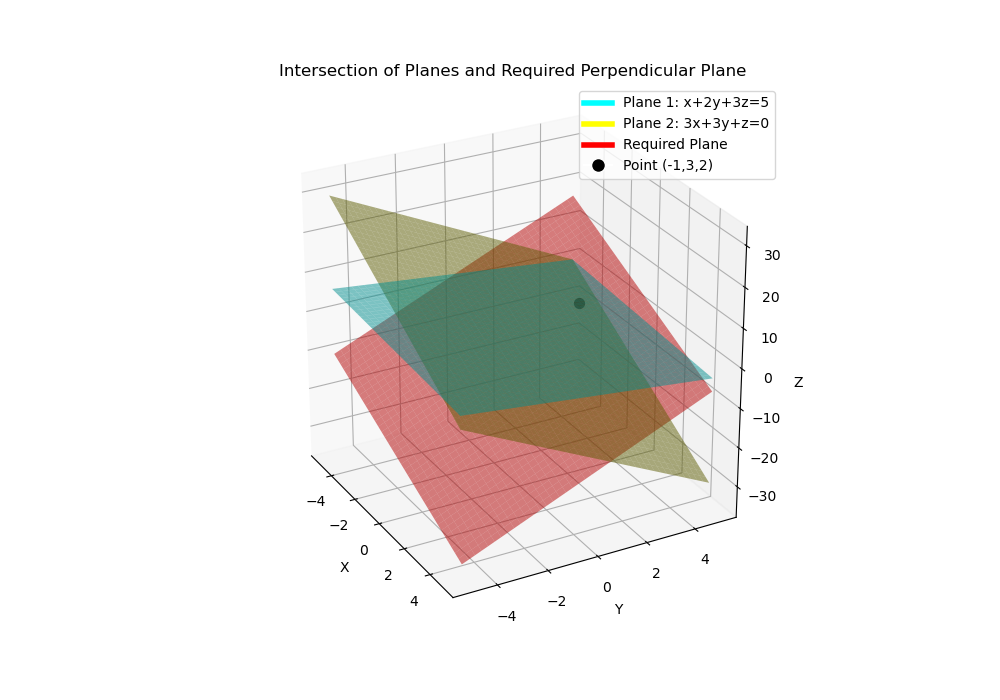
\includegraphics[width=0.9\columnwidth]{../figs/plot8.png}
     \caption*{}
     \label{fig:plot_plane}
 \end{figure}
\end{frame}

\end{document}